

\section{Fluxo de Atividades do Projeto}
\begin{frame}
 \frametitle{Fluxo de Atividades do Projeto}
 \begin{itemize}
  \item Existe uma grande dificuldade das pessoas em saber como começar um projeto
 \end{itemize}
\begin{block}{}
 Como planejar, executar e monitorar um projeto?
\end{block}
\end{frame}

\begin{frame}
 \frametitle{Grupo de processos de iniciação}
 \begin{block}{Objetivo}
  O objetivo principal deste grupo de processos é \textbf{alinhar as expectativas} das partes interessadas com o \textbf{objetivo do projeto}, dar-lhes visibilidade
sobre o \textbf{escopo e objetivos}, e mostrar como a sua participação no projetos e em suas respectivas fases pode assegurar a realização das suas expectativas
 \end{block}

\end{frame}



  \begin{frame}
   \frametitle{Grupo de Processo (“FASE”) – INICIAÇÃO}
   \begin{itemize}
   \item O grupo de processos de iniciação consiste dos processos realizados para definir um novo projeto ou
uma nova fase de um projeto existente por meio da obtenção de autorização para iniciar o projeto ou fase

    \item A documentação para esta decisão também pode conter a declaração inicial do \textbf{escopo} do projeto, \textbf{entregas}, \textbf{duração} do projeto e uma previsão dos \textbf{recursos}
para a análise do investimento da organização
   \end{itemize}

  \end{frame}
  
  \begin{frame}
 \frametitle{Fluxo de Atividades do Projeto}
  \begin{block}{}
   O modelo proposto foi baseado nas teorias propostas no PMBOK, além das considerações de Lewis, Kerzner, Schtub, Galbraith, e Sanders
%   Kerzner \footnote{Kerzer, Harold. Project Management: A system approach to planning sheduling e and controlling; 6ª. Ed; New York; Van Nostrand Reinhold; 1998},
%   Schtub \footnote{Shtub, Avraham & Bard, Jonathan F., Globerson, Shlomo. Project Management-Engineering, Technology and Implementation; New Jersey; Prentice All; 1994},
%   Galbraith \footnote{ Galbraith, Jay R. Desinging Organizations: An Executive Briefing on Strategy, Structure and Process; San Francisco; Jossey-Bass Publishers, 1995},
%   e Sanders \footnote{Sanders, Norman. Stop Wasting Time: Computer-Aided Planning and Control; London; Prentice Hall; 1991}. 
  \end{block}
%    \footnote{Lewis, James P. Project Planning, Scheduling & Control; Chicago; Irwin Professional Publishing; 1995},
\end{frame}

      \begin{frame}
   \frametitle{Grupo de Processo (“FASE”) – INICIAÇÃO}
    \begin{figure}
  \centering
  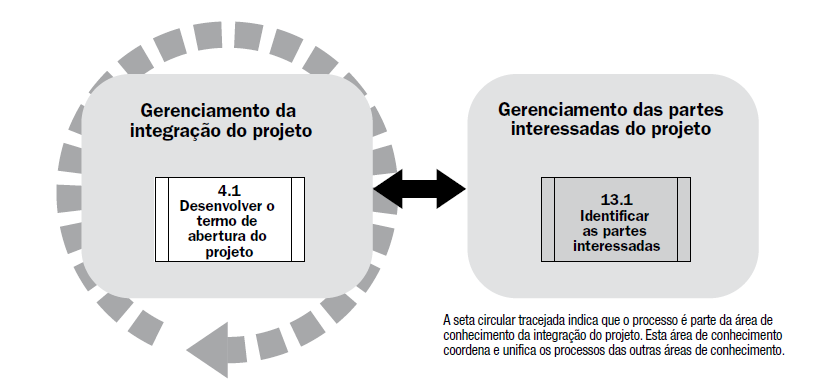
\includegraphics[width = 0.8\textwidth]{figs/fig1_17.png}
  \caption{Grupo de processos de iniciação}
 \end{figure}
  \end{frame}
  
    \begin{frame}
   \frametitle{Fluxo de Atividades do Projeto}
  
   \begin{itemize}
    \item É importante ressaltar, que mesmo sendo um fluxo sequencial, as fases são cíclicas. Elaboração progressiva, incremental e iterativa!
   \end{itemize}

    \begin{figure}
  \centering
  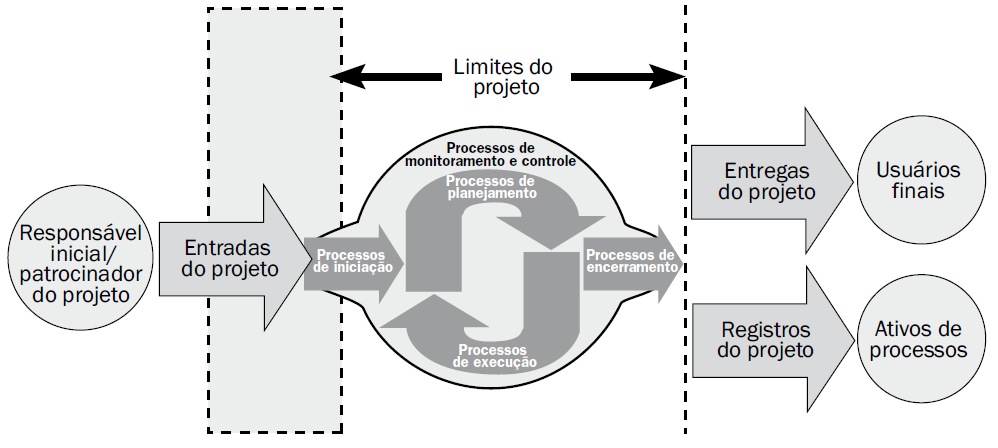
\includegraphics[width = 0.8\textwidth]{figs/fig1_8.png}
  %\caption{A relação entre as partes interessadas do Projeto}
 \end{figure}
  \end{frame}
  
% \begin{frame}
%    \frametitle{Grupo de Processo (“FASE”) – INICIAÇÃO}
%    \begin{figure}
%   \centering
%   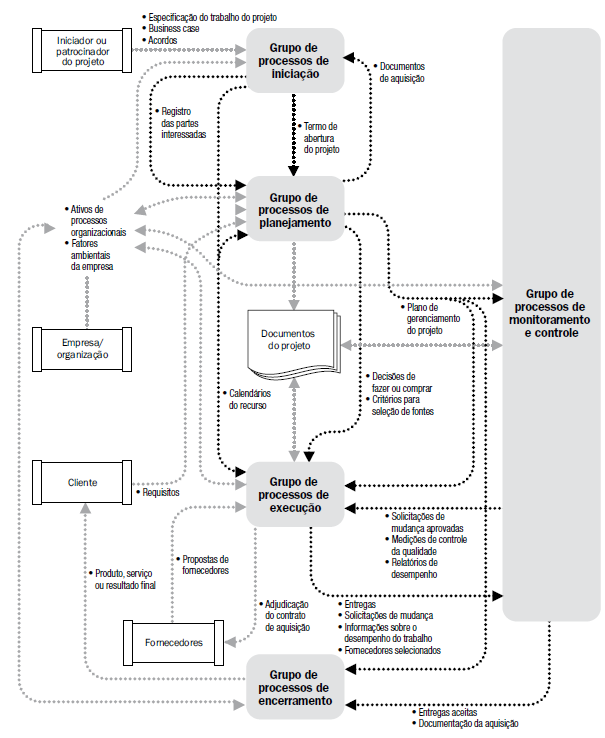
\includegraphics[height = 0.9\textheight]{figs/fig1_10.png}
%   \caption{Fluxograma}
%  \end{figure}
% \end{frame}

\begin{frame}
   \frametitle{Grupo de Processo (“FASE”) – INICIAÇÃO}
   \begin{figure}
  \centering
  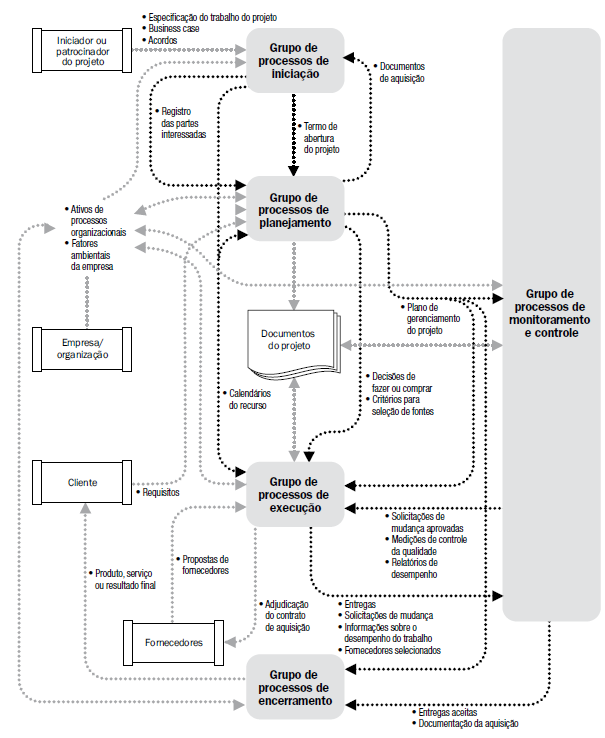
\includegraphics[height = 0.9\textheight]{figs/fig1_10.png}
  %\caption{Fluxograma }
 \end{figure}
\end{frame}
  
  \begin{frame}
   \frametitle{Grupo de Processo (“FASE”) – INICIAÇÃO}
   \begin{figure}
  \centering
  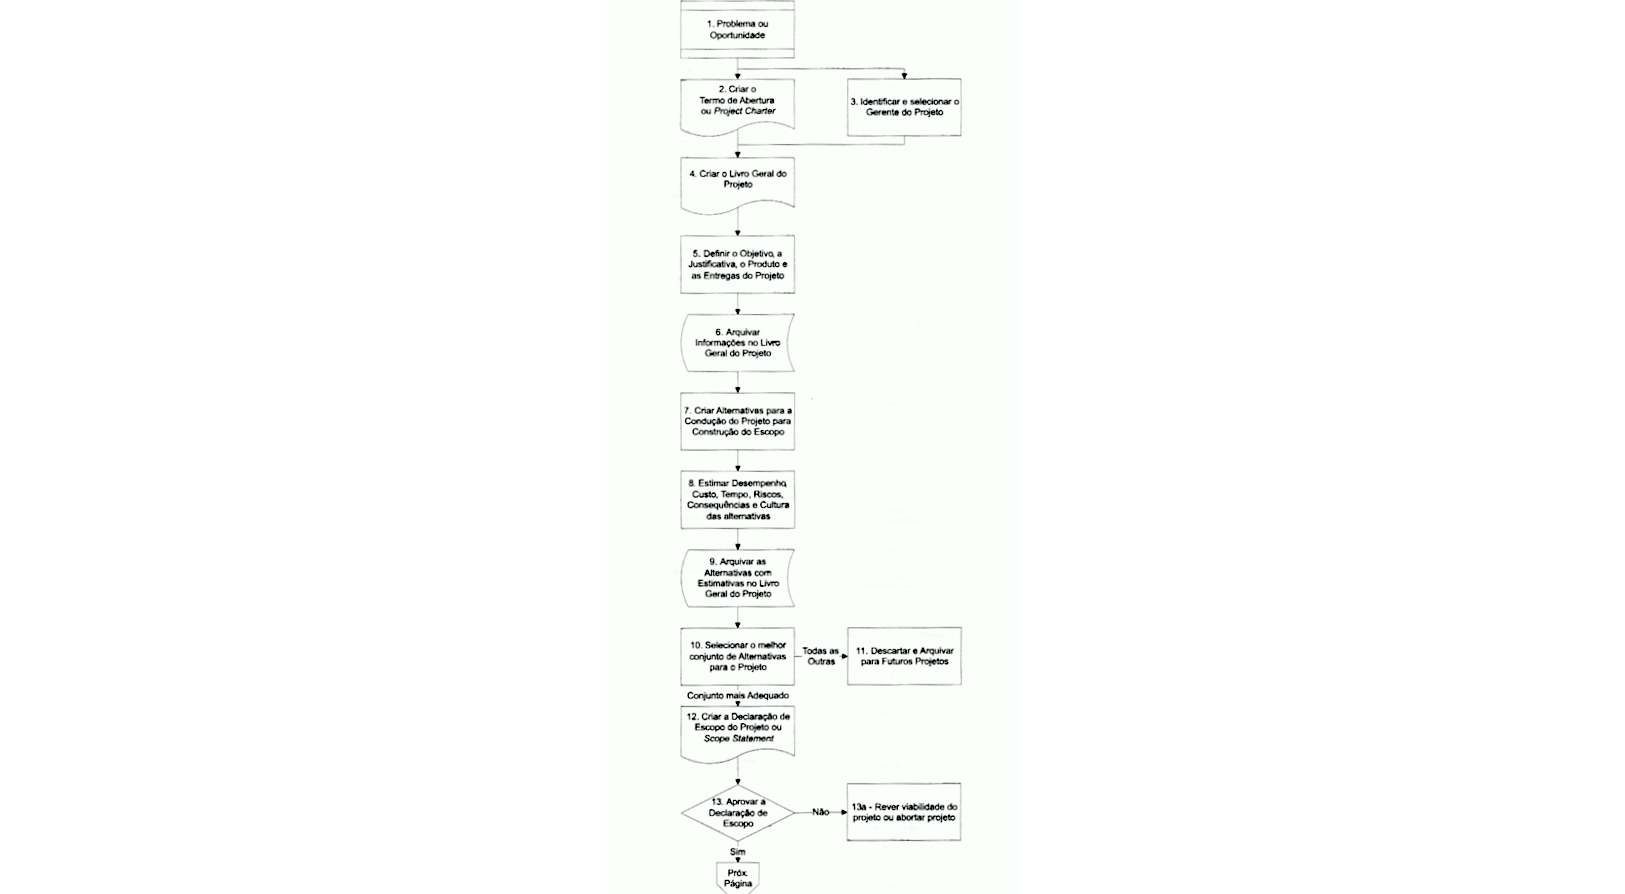
\includegraphics[height = 0.8\textheight]{figs/fig1_14.png}
  \caption{Fluxograma}
 \end{figure}
\end{frame}

 \begin{frame}
   \frametitle{Grupo de Processo (“FASE”) – INICIAÇÃO}
    \begin{figure}
  \centering
  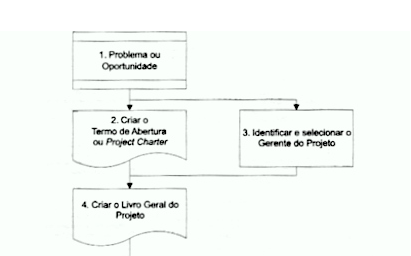
\includegraphics[width = 0.6\textwidth]{figs/fig1_9.png}
  \caption{Fluxograma - Detalhe}
 \end{figure}
  \end{frame}


\begin{frame}
   \frametitle{Grupo de Processo (“FASE”) – INICIAÇÃO}
   \begin{figure}
  \centering
  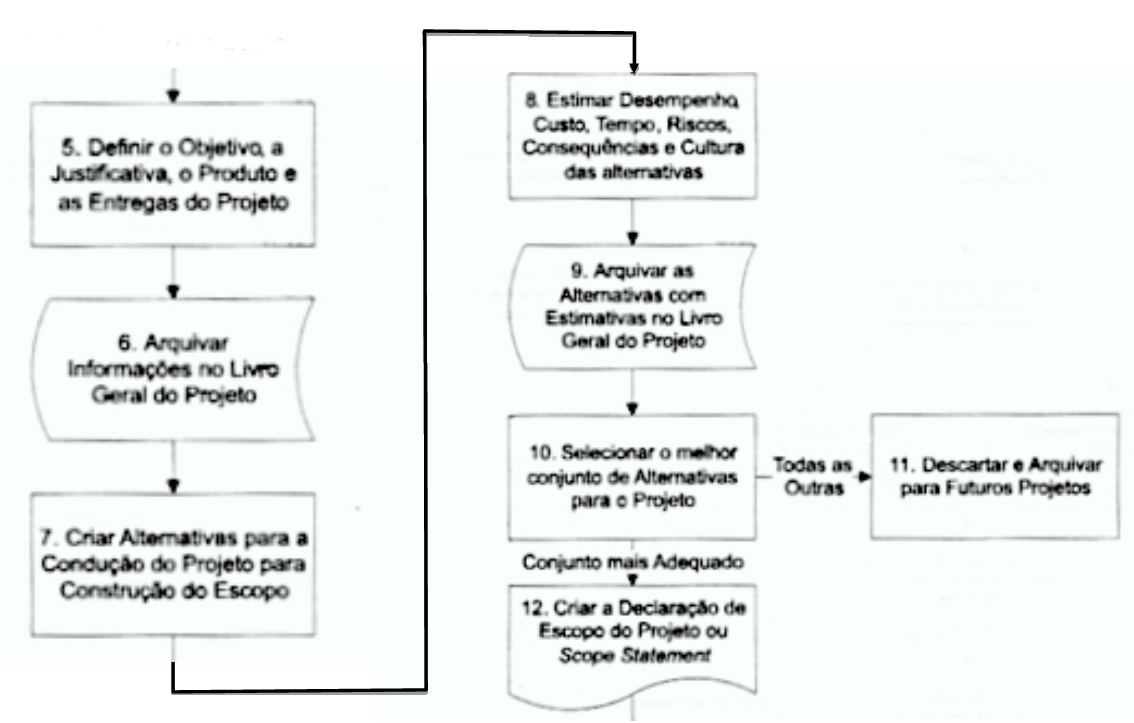
\includegraphics[height = 0.8\textheight]{figs/fig1_16.png}
  \caption{Fluxograma - Detalhe}
 \end{figure}
\end{frame}

\begin{frame}
   \frametitle{Grupo de Processo (“FASE”) – INICIAÇÃO}
   \begin{figure}
  \centering
  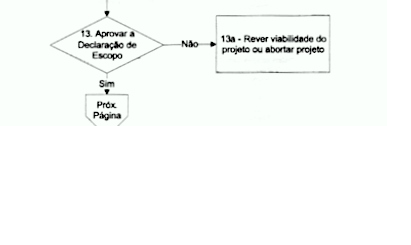
\includegraphics[height = 0.7\textheight]{figs/fig1_15.png}
  \caption{Fluxograma - Detalhe}
 \end{figure}
\end{frame}




% Inserir imagens ruins
\section{Problema ou Oportunidade}
\begin{frame}
   \frametitle{Grupo de Processo (“FASE”) – INICIAÇÃO}
   \begin{itemize}
    \item[1] Problema ou Oportunidade
    \begin{itemize}
     \item Todo projeto tem sua origem em um problema ou oportunidade
     \item Pressões em relação as oportunidades
     \begin{itemize}
      \item Empresas concorrentes
      \item Mercado consumidor
     \end{itemize}
    \end{itemize}
   \end{itemize}
  \begin{block}{}
   Problema é o obstáculo que está entre o local onde se está e o local em que se gostaria de estar
  \end{block}
\end{frame}

\begin{frame}
   \frametitle{Grupo de Processo (“FASE”) – INICIAÇÃO}
  \begin{itemize}
    \item[1] Problema ou Oportunidade
   \begin{itemize}
    \item Pode-se ter como metas a serem atingidas por essa formalização as seguintes
    \begin{itemize}
     \item Identificar e realizar, da melhor forma possível, os esforços necessários para se chegar ao outro lado
     \item Evitar, de todas as formas possíveis, que o obstáculo aumente ou passe a prejudicar outras atividades
     \item Saber avaliar corretamente se o que se quer é realmente chegar ao outro lado
    \end{itemize}
   \end{itemize}
   \end{itemize}
   
\end{frame}

\begin{frame}
   \frametitle{Grupo de Processo (“FASE”) – INICIAÇÃO}
   \begin{itemize}
     \item[1] Problema ou Oportunidade
    \begin{itemize}
     \item Existem basicamente dois tipos de problemas
     \begin{itemize}
      \item \textbf{Problemas de variáveis abertas}
       \item não possuem uma única solução determinada e clara
       \item estão sujeitos a modificações mercadológicas, ambientais e até mesmo a decisões estratégicas da empresa
       \item envolvem a grande maioria dos projetos, principalmente desenvolvimento de software
     \end{itemize}
    \end{itemize}
   \end{itemize}
\end{frame}

\begin{frame}
   \frametitle{Grupo de Processo (“FASE”) – INICIAÇÃO}
   \begin{itemize}
     \item[1] Problema ou Oportunidade
    \begin{itemize}
     \item Existem basicamente dois tipos de problemas
     \begin{itemize}
      \item \textbf{Problemas de variáveis fechadas}
       \item possuem apenas uma única solução matematicamente definida
       \item são aparentemente de controle mais fácil, uma vez que, não sofrem nenhuma influência do ambiente externo
     \end{itemize}
    \end{itemize}
   \end{itemize}
\end{frame}

\section{Livro Geral do Projeto}
\begin{frame}
   \frametitle{Grupo de Processo (“FASE”) – INICIAÇÃO}
   \begin{itemize}
    \item[4] Criar o Livro Geral do Projeto
    \begin{itemize}
     \item É importante que todas as informações do projeto sejam documentadas
     \begin{itemize}
      \item Registrar, formalmente, as decisões e aprovações dos envolvidos (assinaturas, observações,…)
     \end{itemize}
    \item Pode ser papel ou eletrônico
     \end{itemize}
   \end{itemize}
\end{frame}

\begin{frame}
   \frametitle{Grupo de Processo (“FASE”) – INICIAÇÃO}
   \begin{itemize}
    \item[4] Criar o Livro Geral do Projeto
    \begin{itemize}
     \item Soluções GED (Gerenciamento Eletrônico de Documentos)  podem ser utilizadas
     \begin{itemize}
      \item Garantem as características de armazenamento e segurança
      \item Converte informações de texto, voz e imagens para a forma digital
     \end{itemize}
     \end{itemize}
   \end{itemize}
   \begin{figure}
    \centering
    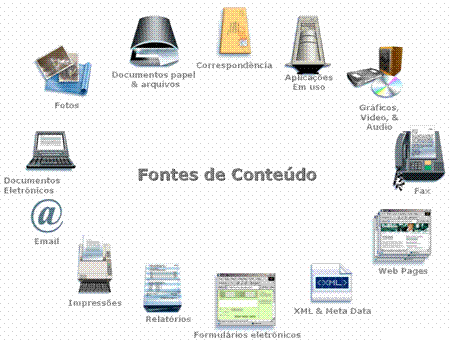
\includegraphics[width = 0.5\textwidth]{figs/fig1_11.png}
   \end{figure}
\end{frame}

\begin{frame}
   \frametitle{Grupo de Processo (“FASE”) – INICIAÇÃO}
   \begin{itemize}
    \item[4] Criar o Livro Geral do Projeto
    \begin{itemize}
     \item Algumas ferramentas
     \begin{itemize}
      \item Project Server (Microsoft)
      \item Redmine
      \item Sites (ex: Wiki) + “SVN”
      \item Redes Sociais específicas para o projeto
      \item Soluções de  Data Warehouse (DW) - Pentaho
     \end{itemize}
     \end{itemize}
   \end{itemize}
\end{frame}
\section{Definir objetivo, justificativa, produtos e entregas}
\begin{frame}
   \frametitle{Grupo de Processo (“FASE”) – INICIAÇÃO}
   \begin{itemize}
    \item[5] DEFINIR O OBJETIVO, A JUSTIFICATIVA, O PRODUTO E AS ENTREGAS
    \begin{block}{}
     Objetivo é a representação formal daquilo que se quer atingir com o término do projeto. É de fácil mensuração!
    \end{block}

    \begin{itemize}
     \item Ex: Implantar práticas ágeis no desenvolvimento de software, no prazo de 2 anos, a partir de 2012, e com um custo estimado de $R\$ 1.000.000,00$
   \end{itemize}
   \end{itemize}
\end{frame}

\begin{frame}
   \frametitle{Grupo de Processo (“FASE”) – INICIAÇÃO}
   \begin{itemize}
    \item[5] DEFINIR O OBJETIVO, A JUSTIFICATIVA, O PRODUTO E AS ENTREGAS
      \begin{itemize}
     \item O objetivo sozinho não define o projeto. É preciso que esteja associado a uma determinada justificativa
     \item Por outro lado, uma determinada justificativa também pode caracterizar inúmeros objetivos
   \end{itemize}
   \end{itemize}
\end{frame}

\begin{frame}
   \frametitle{Grupo de Processo (“FASE”) – INICIAÇÃO}
   \begin{itemize}
    \item[5] DEFINIR O OBJETIVO, A JUSTIFICATIVA, O PRODUTO E AS ENTREGAS
    \begin{block}{}
    Produtos são os resultados obtidos na conclusão do projeto
    \end{block}

    \begin{itemize}
     \item Ex: Ferramenta de análise estática de código instalada e customizada, além de equipe treinada
     \item Ex: Ferramenta de integração contínua instalada e customizada, além de equipe treinada
   \end{itemize}
   \end{itemize}
\end{frame}

\begin{frame}
   \frametitle{Grupo de Processo (“FASE”) – INICIAÇÃO}
   \begin{itemize}
    \item[5] DEFINIR O OBJETIVO, A JUSTIFICATIVA, O PRODUTO E AS ENTREGAS
    \begin{block}{}
    Entregas são todos os resultados físicos ou semiprodutos obtidos ao longo do projeto
    \end{block}

    \begin{itemize}
     \item Ex: Processo customizado na ferramenta EPF  (Eclipse Process Framework Composer)
     \item Ex: Release 4.1.32
     \item Ex: Backlog de Produto
     \item Ex: Relatórios de desempenho
   \end{itemize}
   \end{itemize}
\end{frame}
\section{Alternativas de Solução}
\begin{frame}
   \frametitle{Grupo de Processo (“FASE”) – INICIAÇÃO}
   \begin{itemize}
    \item[7] CRIAR ALTERNATIVAS DE SOLUÇÃO
    \begin{block}{}
   Como iremos fazer isso?
    \end{block}

    \begin{itemize}
     \item Aternativas devem ser capazes de responder a pergunta
     \item Diversos fatores devem ser considerados
     \begin{itemize}
      \item \textbf{Ambientais}: tecnologia, economia, governo, sociedade,...
      \item \textbf{Organizacionais}: experiência da equipe, relações de trabalho, comprometimento da organização com o projeto,...
     \end{itemize}
   \end{itemize}
   \end{itemize}
\end{frame}

\begin{frame}
   \frametitle{Grupo de Processo (“FASE”) – INICIAÇÃO}
   \begin{itemize}
    \item[7] CRIAR ALTERNATIVAS DE SOLUÇÃO
    \begin{block}{}
   Como iremos fazer isso?
    \end{block}

    \begin{itemize}
     \item A expectativa da alta gerência e dos usuários , é a maior influenciadora do sucesso ou do fracasso do projeto
     \item As alternativas iniciais são vagas e imprecisas. Por outro lado, se identificadas tardiamente, as decisões normalmente já foram tomadas
     \item Use Brainstorming para identificar as alternativas!
   \end{itemize}
   \end{itemize}
\end{frame}

\begin{frame}
   \frametitle{Grupo de Processo (“FASE”) – INICIAÇÃO}
   \begin{itemize}
    \item[7] CRIAR ALTERNATIVAS DE SOLUÇÃO
   \end{itemize}
   \begin{figure}
    \centering
    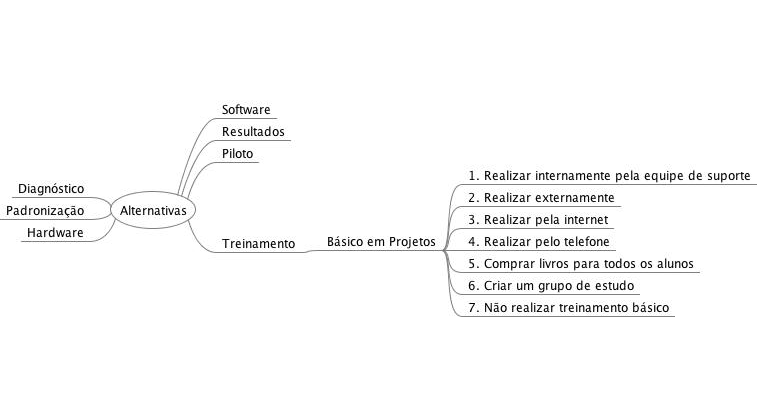
\includegraphics[width = 0.8\textwidth]{figs/fig1_13.png}
   \end{figure}
\end{frame}
\section{Estimar}
\begin{frame}
 \frametitle{Grupo de Processo (“FASE”) – INICIAÇÃO}
 \begin{itemize}
  \item[8] ESTIMAR DESEMPENHO, CUSTO, TEMPO, RISCOS, CONSEQUENCIAS E CULTURA DAS ALTERNATIVAS
  \begin{itemize}
   \item Cada alternativa deve ser estimada
   \item Estimativas, por serem empíricas, atribuir notas (0 a 10). Quanto mais próxima de 10, mais atenderá ao objetivo
   \item Fatores a serem analisados
   \begin{itemize}
    \item Desempenho (P)
    \item Custos (C)
    \item Tempo (T)
    \item Riscos (R)
    \item Consequencias (CO)
    \item Adequação à Cultura (AC)
   \end{itemize}

  \end{itemize}

 \end{itemize}

\end{frame}


\begin{frame}
 \frametitle{Grupo de Processo (“FASE”) – INICIAÇÃO}
 \begin{itemize}
  \item[8] SELECIONAR O MELHOR CONJUNTO DE ALTERNATIVAS PARA O PROJETO
 \end{itemize}

    \begin{figure}
    \centering
    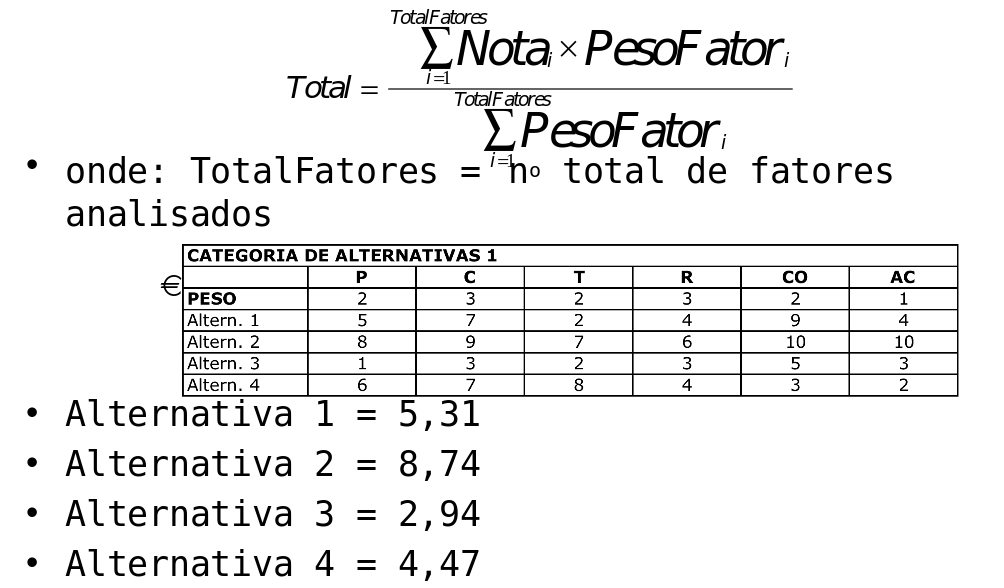
\includegraphics[width = 0.9\textwidth]{figs/fig1_12.png}
   \end{figure}
\end{frame}

\section{Exercício}
\begin{frame}
 \frametitle{Exercício}
 \begin{itemize}
  \item Identifique quais são as atividades que ainda precisam ser refinadas ou realizadas no projeto da disciplina, a partir do fluxograma da “fase”de Iniciação
 \end{itemize}
\end{frame}

\section{Bibliografia}
\begin{frame}
 \frametitle{Bibliografia}
 \begin{itemize}
  \item Lewis, James P. Project Planning, Scheduling \& Control; Chicago; Irwin Professional Publishing; 1995
  \item Kerzer, Harold. Project Management: A system approach to planning sheduling e and controlling; 6. Ed; New York; Van Nostrand Reinhold; 1998
  \item Shtub, Avraham \& Bard, Jonathan F., Globerson, Shlomo. Project Management-Engineering, Technology and Implementation; New Jersey; Prentice All; 1994
  \item  Galbraith, Jay R. Desinging Organizations: An Executive Briefing on Strategy, Structure and Process; San Francisco; Jossey-Bass Publishers, 1995
 
  \end{itemize}
\end{frame}

\begin{frame}
 \frametitle{Bibliografia e Leitura Sugerida}
 \begin{itemize}
  \item Sanders, Norman. Stop Wasting Time: Computer-Aided Planning and Control; London; Prentice Hall; 1991
  \item Modelos Hibridos - Proxima tendencia em gerenciamento de projetos \url{http://www.mundopm.com.br/images/editorialEd64.pdf}
  \end{itemize}
\end{frame}